\documentclass[12pt]{article}
\usepackage{amsmath}  % Math
\usepackage{amssymb}  % Symbols
\usepackage{graphicx} % Images
\usepackage[utf8]{inputenc}
\usepackage[T1]{fontenc}
\usepackage[margin=1in]{geometry}
\usepackage[spanish]{babel}
\usepackage{transparent}
\usepackage{eso-pic}
\usepackage{xcolor}
\usepackage{subcaption} % For subfigures

\graphicspath{{images/}} % Path to images
\newcommand\BackgroundPic{
    \put(0,0){
        \parbox[b][\paperheight]{\paperwidth}{
            \vfill
            \centering
            \transparent{0.1}
\includegraphics[width=\paperwidth]{logo} % your image
            \vfill
        }
    }
}


\title{Informe Negocio Empanadas: \\
\textit{Las Empanadas Hermanas}} % Title of the report
  \author{Autores: Felipe Colli, Juan Gonzalez, Bastián Ortiz y Javier Robles \thanks{Instituto Nacional General José Miguel Carrera} \\
  Curso: \textit{4°H}, Profesor: \textit{Carlos Morales}} % Add your names and course
  \date{30 de mayo de 2025} % Fecha de Entrega
\AddToShipoutPicture{\BackgroundPic} % Add background image

\begin{document}

\maketitle
\begin{figure}[h!] % Use [h!] or [htbp] for better float placement
    \centering
    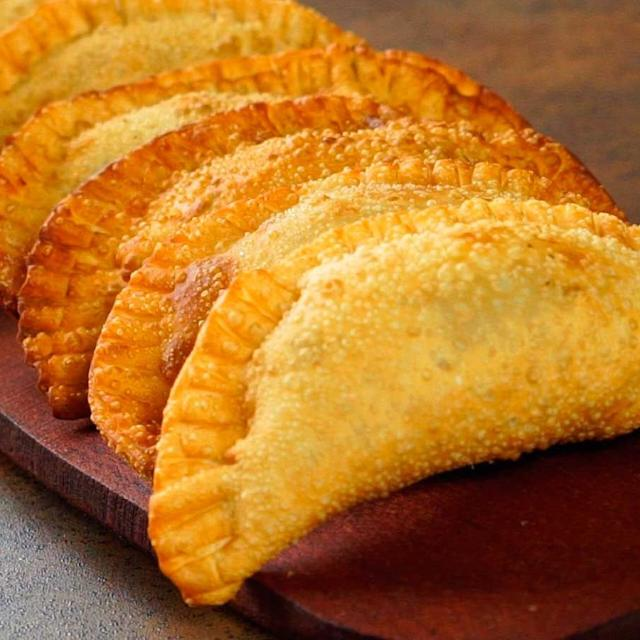
\includegraphics[width=0.8\textwidth]{empanadas} % Logo of the school
\end{figure}
\newpage

\tableofcontents
\newpage

\section{Resumen} % Aprox 1/3 de Pagina
% Content for Resumen
\newpage



\section{Introducción} % Max 1 pagina
El presente informe tiene como objetivo presentar el negocio de empanadas "Las Empanadas Hermanas", un emprendimiento que busca ofrecer empanadas de alta calidad. A través de este documento, se detallarán los aspectos clave del negocio, incluyendo su propuesta de valor, mercado objetivo y proyecciones financieras iniciales correspondientes al primer avance del trabajo de Matemática Financiera. \\

Dentro de las proyecciones financieras, se contempla un análisis de costos y precios para una producción inicial, así como una estimación de las ganancias esperadas. El negocio se enfoca en la producción y venta de tres variedades principales de empanadas: Pino (carne), Queso Clásica, y Camarón Queso, con un énfasis en la calidad de los ingredientes y la satisfacción del cliente. Todo esto se desarrolla sin olvidar el marco legal regulatorio, por lo cual este negocio no será un frente para lavado de activos, evasión de impuestos, generación de facturas ideológicamente falsas, o la venta de drogas ilícitas. \\ % Referencia a Breking Bad y Los Pollos Hermanos. Mantener el toque estudiantil.


\subsection{Objetivos del Negocio:}
\begin{enumerate}
    \item \textbf{Propuesta de Valor Inicial:} Ofrecer tres variedades de empanadas (Pino, Queso, Camarón Queso) de alta calidad, elaboradas con ingredientes frescos, destacando el sabor tradicional.
    \item \textbf{Estimación de Producción y Ventas:} Definir una cantidad inicial de productos a vender para el primer mes (500 unidades por variedad, total 1500 empanadas).
    \item \textbf{Análisis de Costos de Ingredientes:} Cotizar los ingredientes en al menos dos proveedores y seleccionar los más convenientes para elaborar una lista de compras detallada y valorizada.
    \item \textbf{Gestión de IVA en Compras:} Elaborar una factura de compra simulada que refleje el valor neto de los ingredientes, el IVA crédito fiscal y el total pagado.
    \item \textbf{Estrategia de Precios y Proyección de Ingresos:} Definir precios de venta competitivos para cada variedad, que cubran costos y generen ganancia. Calcular el ingreso total neto esperado y el IVA débito fiscal.
    \item \textbf{Cálculo de Obligaciones Tributarias (IVA):} Determinar el monto de IVA a pagar al fisco, resultante de la diferencia entre IVA débito e IVA crédito.
    \item \textbf{Evaluación de Rentabilidad Inicial:} Calcular las ganancias del primer mes y verificar si son suficientes para reinvertir en la producción del mes siguiente y obtener un excedente (sueldo para el grupo).
    \item \textbf{Viabilidad del Negocio (Preliminar):} Evaluar la viabilidad preliminar del negocio basándose en los cálculos financieros del primer mes de operación.

\end{enumerate}

\newpage



\section{Desarrollo} % 2 - 5 paginas

\subsection{Tabla de Costos Ingredientes}

\begin{table}[h!]
    \centering
    \begin{tabular}{|| c | c | c | c||} 
        \hline
    \textbf{Distribuidor} & Formato & \textbf{Costo} & \textbf{Costo 100 Unidades} \\ [0.5ex]
        \hline\hline
        \multicolumn{4}{||c||}{\textbf{Masa Prehecha Grande}} \\ [0.5ex] \hline \hline
        El Palacio de las Empanadas & 20 Un & \$4100 & \$20500 \\ \hline
        Masas Mi Tierra & 25 Un & \$8000 & \$31000 \\ \hline
        Alimentos La Kosa & 20 Un & \$4200 & \$21000 \\ [1ex] \hline \hline

        \multicolumn{3}{||c||}{\textbf{Huevos}} & \textbf{Costo por Docena} \\ [0.5ex] \hline \hline
        El Don Huevo & 180 Un & \$39500 & \$2633 \\ \hline
        Huevos La Montaña Pelluhue & 180 Un & \$43990 & \$2932 \\ \hline
        AgricoVial & 180 Un & \$41600 & \$2773 \\ [1ex] \hline \hline

        \multicolumn{3}{||c|}{\textbf{Camaron}} & \textbf{Costo por KG} \\ [0.5ex] \hline \hline
        Distribuidora GK & 10 KG & \$48900 & \$4890 \\ \hline
        Comercial Oceanica & 10 KG & \$55800 & \$5580 \\ \hline
        Del Origen & 10 KG & \$48700 & \$4870 \\ [1ex] \hline \hline

        \multicolumn{3}{||c|}{\textbf{Carne Molida}} & \textbf{Costo por KG} \\ [0.5ex] \hline \hline % Added Costo por KG header for consistency
        Central Mayorista & 500 G & \$2590 & \$5080 \\ \hline 
        Unimarc & 1 KG & \$4990 & \$4990 \\ \hline 
        El Paiquito & 250 G & \$1090 & \$4360 \\ [1ex] \hline \hline


        \multicolumn{3}{||c|}{\textbf{Queso}} & \textbf{Costo por KG} \\ [0.5ex] \hline \hline % Added Costo por KG header
        Distribuidora Santiago & 1 KG & \$9580 & \$9580 \\ \hline
        Distribuidora Nueva de Matte & 1 KG & \$6940 & \$6940 \\ \hline
        Mayorista 10 & 1 KG & \$9160 & \$9160 \\ [1ex] \hline \hline

        \multicolumn{3}{||c|}{\textbf{Cebolla}} & \textbf{Costo por KG} \\ [0.5ex] \hline \hline % Added Costo por KG header
        Santiago Natural Foods & 14 KG & \$10990 & \$785 \\ \hline
        Distribuidora Frest & 10 KG & \$9990 & \$990 \\ \hline
        Lider & 1 KG & \$1195 & \$1195 \\ [1ex] \hline \hline

        \multicolumn{3}{||c|}{\textbf{Aceite}} & \textbf{Costo por Litro} \\ [0.5ex] \hline \hline
        ProsudMarket & 18 L & \$39614 & \$2200.77 \\ \hline
        Central Mayorista & 13.5 L & \$22200 & \$1644.44 \\ \hline
        Distribuidora Sabatini & 5L & \$9296 & \$1859.20 \\ [1ex] \hline \hline

    \end{tabular}
    \caption{Tabla de Costos de Ingredientes}
    \label{tab:costos_ingredientes}
\end{table} %Fin Priemra Pagina del Desarrollo
\newpage


\subsection{Cotizaciones Ingredientes}
    %\subsubsection{Masa Prehecha}
        \begin{figure}[h!] % Use [h!] or [htbp] for better float placement
            \centering % Center the content of the figure
            \begin{subfigure}{0.4\textwidth}
                \centering
                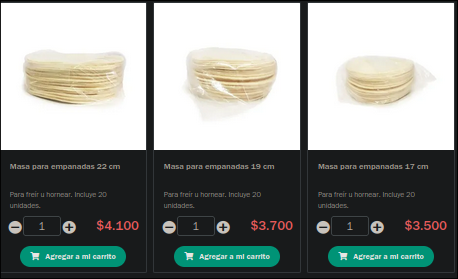
\includegraphics[width=0.9\linewidth]{palaci} % Removed space before ]
                \caption{Palacio de las Empanadas}
                \label{fig:palacio}
            \end{subfigure}
            \hfill % Add some space between subfigures
            \begin{subfigure}{0.4\textwidth}
                \centering
                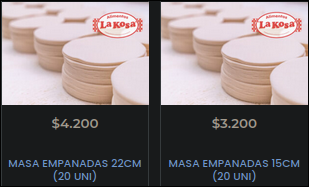
\includegraphics[width=0.9\linewidth]{kosa} % Removed space before ]
                \caption{Alimentos La Kosa}
                \label{fig:kosa}
            \end{subfigure}
            \caption{Cotizaciones de Distribuidores de Masa Prehecha}
            \label{fig:cotizaciones_masas}
        \end{figure} % END OF THIS FIGURE

    %\subsubsection{Huevos}
        \begin{figure}[h!] % START A NEW FIGURE
            \centering
            \begin{subfigure}{0.35\textwidth}
                \centering
                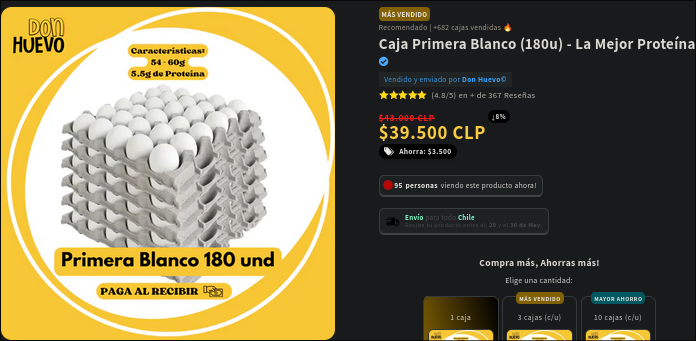
\includegraphics[width=0.9\linewidth]{donhuevo} % Removed space before ]
                \caption{El Don Huevo}
                \label{fig:don_huevo}
            \end{subfigure}
            \hfill
            \begin{subfigure}{0.4\textwidth}
                \centering
                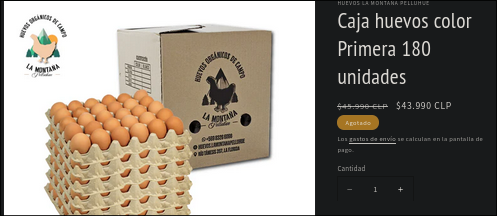
\includegraphics[width=0.9\linewidth]{montan1} % Removed space before ]
                \caption{Huevos La Montaña Pelluhue}
                \label{fig:huevos_montaña}
            \end{subfigure}
            \caption{Cotizaciones de Distribuidores de Huevos}
            \label{fig:cotizaciones_huevos}
        \end{figure} % END OF THIS FIGURE

    %\subsubsection{Camaron}
        \begin{figure}[h!] % START A NEW FIGURE
            \centering
            \begin{subfigure}{0.4\textwidth}
                \centering
                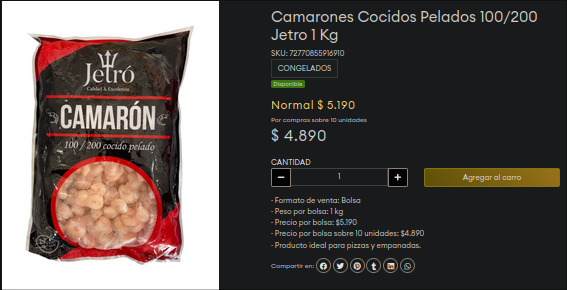
\includegraphics[width=0.9\linewidth]{gk} % Removed space before ]
                \caption{Distribuidora GK}
                \label{fig:distribuidora_gk}
            \end{subfigure}
            \hfill
            \begin{subfigure}{0.35\textwidth}
                \centering
                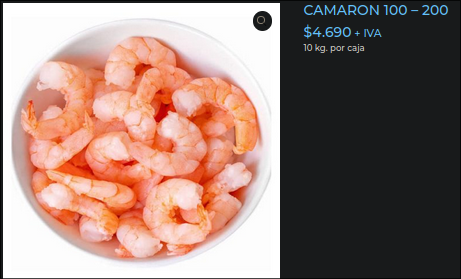
\includegraphics[width=0.9\linewidth]{oceanic} % Removed space before ]
                \caption{Comercial Oceanica}
                \label{fig:comercial_oceanica}
            \end{subfigure}
            \caption{Cotizaciones de Distribuidores de Camarón}
            \label{fig:cotizaciones_camaron}
        \end{figure} % END OF THIS FIGURE
        %\newpage % You can uncomment this if you specifically want a page break herei
        % Fin segunda pagina del desarrollo

    %\subsubsection{Carne Molida}
        \begin{figure}[h!] % START A NEW FIGURE
            \centering
            \begin{subfigure}{0.45\textwidth}
                \centering
                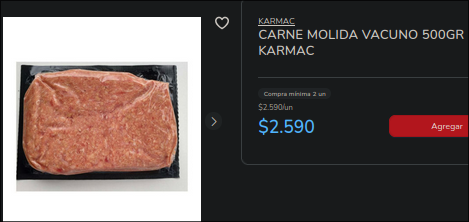
\includegraphics[width=0.9\linewidth]{central} % Removed space before ]
                \caption{Central Mayorista}
                \label{fig:central_mayorista}
            \end{subfigure}
            \hfill
            \begin{subfigure}{0.45\textwidth}
                \centering
                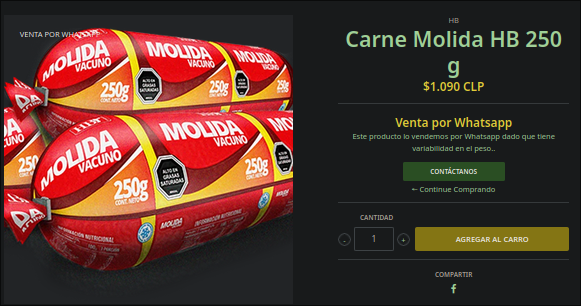
\includegraphics[width=0.9\linewidth]{paiquito} % Removed space before ]
                \caption{Paiquito}
                \label{fig:unimarc} % Consider if fig:paiquito is a more suitable label
            \end{subfigure}
            \caption{Cotizaciones de Distribuidores de Carne Molida}
            \label{fig:cotizaciones_carne_molida}
        \end{figure} % END OF THIS FIGURE

    %\subsubsection{Queso}
        \begin{figure}[h!] % START A NEW FIGURE
            \centering
            \begin{subfigure}{0.45\textwidth}
                \centering
                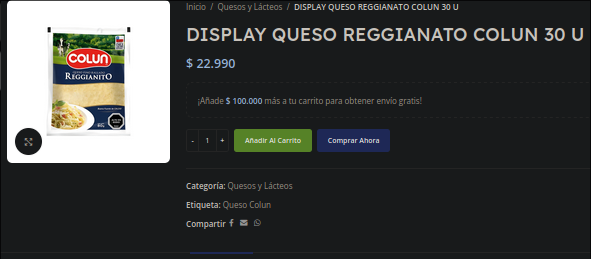
\includegraphics[width=0.9\linewidth]{santiago} % Removed space before ]
                \caption{Distribuidora Santiago}
                \label{fig:distribuidora_santiago}
            \end{subfigure}
            \hfill
            \begin{subfigure}{0.45\textwidth}
                \centering
                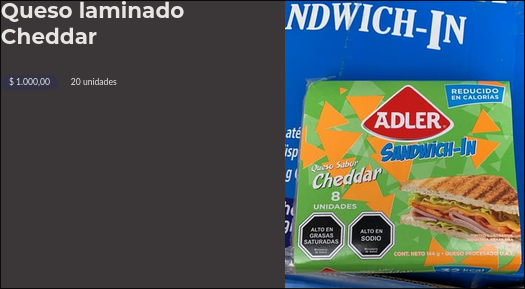
\includegraphics[width=0.9\linewidth]{nueva} % Removed space before ]
                \caption{Distribuidora Nueva de Matte}
                \label{fig:distribuidora_nueva_de_matte}
            \end{subfigure}
            \caption{Cotizaciones de Distribuidores de Queso}
            \label{fig:cotizaciones_queso}
        \end{figure} % END OF THIS FIGURE

    %\subsubsection{Cebolla}
        \begin{figure}[h!] % START A NEW FIGURE
            \centering
            \begin{subfigure}{0.4\textwidth}
                \centering
                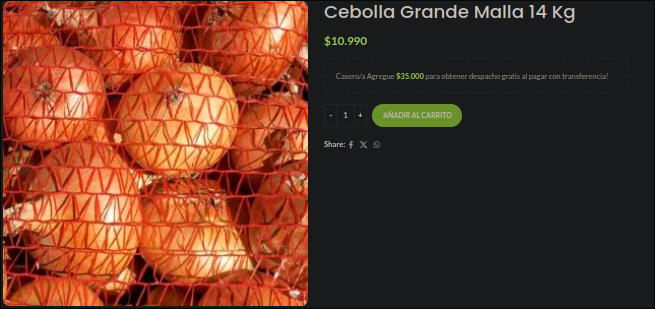
\includegraphics[width=0.9\linewidth]{nat} % Removed space before ]
                \caption{Santiago Natural Foods}
                \label{fig:santiago_natural_foods}
            \end{subfigure}
            \hfill
            \begin{subfigure}{0.45\textwidth}
                \centering
                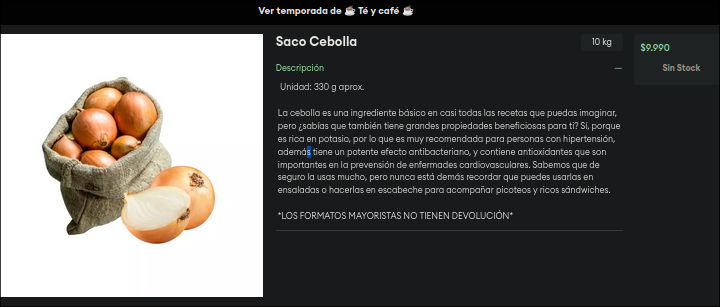
\includegraphics[width=0.9\linewidth]{fres} % Removed space before ]
                \caption{Distribuidora Frest}
                \label{fig:distribuidora_frest}
            \end{subfigure}
            \caption{Cotizaciones de Distribuidores de Cebolla}
            \label{fig:cotizaciones_cebolla}
        \end{figure} % END OF THIS FIGURE

    %\subsubsection{Aceite}
        \begin{figure}[h!] % START A NEW FIGURE
            \centering
            \begin{subfigure}{0.45\textwidth}
                \centering
                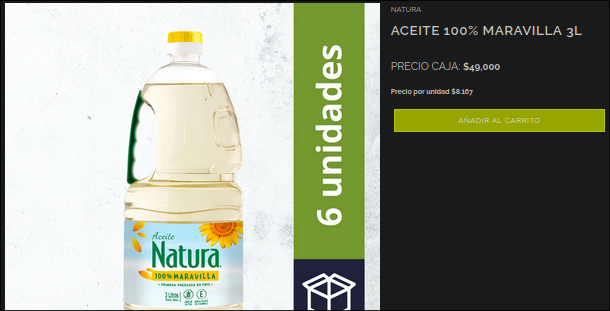
\includegraphics[width=0.9\linewidth]{prosud} % Removed space before ]
                \caption{ProsudMarket}
                \label{fig:prosudmarket}
            \end{subfigure}
            \hfill
            \begin{subfigure}{0.45\textwidth}
                \centering
                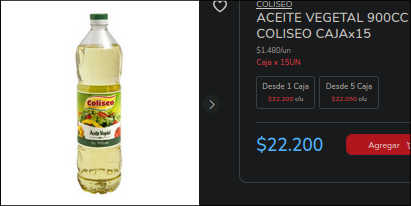
\includegraphics[width=0.9\linewidth]{aceite} % Removed space before ]
                \caption{Central Mayorista}
                \label{fig:central_mayorista_aceite}
            \end{subfigure}
            \caption{Cotizaciones de Distribuidores de Aceite}
            \label{fig:cotizaciones_aceite}
        \end{figure} % END OF THIS FIGURE
        % Fin tercera pagina del desarrollo
        
        \newpage % This newpage was already here, affecting layout before Conclusiones
        \[\transparent{0}\]

    \subsection{Facturas e IVA} %tengo 2 paginas para hacer todo hasta antes d ela conlusion, ns como chucha lo haremos 🥵
        \subsubsection{Lista a Comprar}
        \subsubsection{Factura de Compra}


    \subsection{Definición de Precios y Proyección de Ingresos}
        \subsubsection{Definición de Precios}
        \subsubsection{Cálculo de Obligaciones Tributarias (IVA)}
        \subsubsection{Proyección de Ingresos}
        
    \newpage


\section{Conclusiones} % Max 1 pagina
% Content for Conclusiones


\end{document}
